%!TEX root = ../template.tex
%%%%%%%%%%%%%%%%%%%%%%%%%%%%%%%%%%%%%%%%%%%%%%%%%%%%%%%%%%%%%%%%%%%%
%% chapter4.tex
%% NOVA thesis document file
%%
%% Chapter with lots of dummy text
%%%%%%%%%%%%%%%%%%%%%%%%%%%%%%%%%%%%%%%%%%%%%%%%%%%%%%%%%%%%%%%%%%%%
\chapter{Diseño de una Red SD-WAN}
\label{cha:Diseño de una Red SD-WAN}

\section{Selección de Proveedor y Tecnología} % (fold)
\label{sec:Selección de Proveedor y Tecnología}

Para la selección de la solución específica que se diseña tenemos en cuenta los costos de cada una de ella y por supuesto las ventajas en términos de servicio que obtendría el cliente, el principal criterio de selección es utilizar la solución que cumpla con los objetivos del proyecto sin implicar costos demasiado grandes para el cliente. Teniendo esto en cuenta debemos considerar la solución actual del cliente.
\\
\\
Hace poco tiempo el cliente migró su infraestructura de unos equipos Mikrotik a dispositivos Cisco, por lo que de ser posible el proyecto debe conservar dichos equipos para no perder la inversión realizada por el cliente. La migración realizada fue de equipos Mikrotik a equipos Cisco 891 en las diferentes tiendas y equipos Cisco 4331 en las regionales y la sede nacional.
\\
\\
Dados los criterios definidos anteriormente se procede a analizar cada una de las soluciones que se plantearon para el desarrollo del proyecto.
\\
\\
La primera opción que se consideró fue utilizar OpenDayLight como controlador SD-WAN ya que este utiliza totalmente software abierto para su funcionamiento, esta plataforma utiliza protocolos abiertos como  Openflow y Netconf, \textbf{Ver figura 9.1 Solución de la Arquitectura}.



\begin{figure}[htbp]
  \centering
  %\subcaptionbox{\label{fig:leftsubfig}}%
    {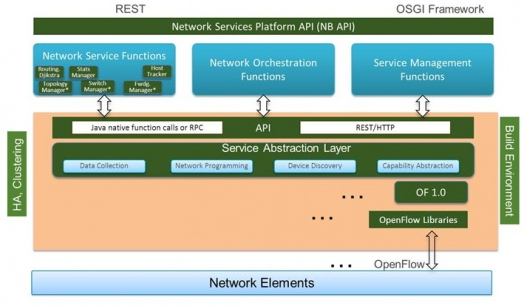
\includegraphics[width=0.9\linewidth]{figure31}}%
%  \subcaptionbox{Another sub-figure\label{fig:rightsubfig}}%
%    {
\includegraphics[width=0.5\linewidth]{knitting-vectorial}}%
  \caption{Solución de la Arquitectura}
  \label{fig:fig2subfig}
\end{figure}

Esta arquitectura aunque al utilizar protocolos estándar permite que se conecte cualquier elemento de red que hable Openflow tiene la limitante de que los equipos de red tradicionales, incluyendo los que tiene el cliente no soportan OpenFlow por defecto, y por tanto los enrutadores que utiliza el cliente hoy en día no se integran con esta arquitectura de SDN, lo que significa que implementar esta solución requeriría cambiar todos los enrutadores por unos que soporten OpenFlow.
\\
\\
Se tuvieron en cuenta también soluciones de varios fabricantes para el proyecto, más precisamente las soluciones SD-WAN de Nokia(Nuage), Cisco(Viptela), vmware(Velo cloud) y Silverpeak, estas son las soluciones que dominan el mercado a la fecha de elaboración de este documento. Todas estas son soluciones SDN \textbf{Ver figura 9.2 Solución y Funcionamiento de una red SD-WAN}. que desagregan completamente los planos de control y gestión de los enrutadores en las sedes Branch y los centralizan en controladoras y servidores de gestión, aunque todas las soluciones mencionadas utilizan protocolos diferentes su arquitectura y funcionamiento es muy similar.
\begin{figure}[htbp]
  \centering
  %\subcaptionbox{\label{fig:leftsubfig}}%
    {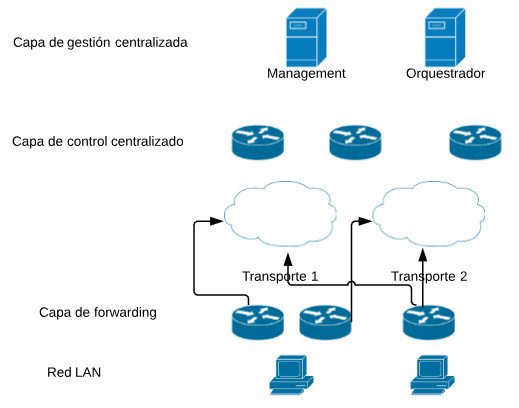
\includegraphics[width=0.9\linewidth]{figure32}}%
%  \subcaptionbox{Another sub-figure\label{fig:rightsubfig}}%
%    {
\includegraphics[width=0.5\linewidth]{knitting-vectorial}}%
  \caption{Solución y Funcionamiento de una red SD-WAN}
  \label{fig:fig2subfig}
\end{figure}
Dentro de cada una de estas opciones se desagregan las capas de control y de gestión en un sitio centralizado, normalmente un centro de datos, y en los branch solamente se tiene la capa de envío de datos o forwarding, estas sedes remotas se comunican entre ellas en todos los casos mediante túneles que se forman automáticamente gracias al plano de control centralizado, sin embargo la tecnología con la que se forman dichos túneles y con la que se envía la información de enrutamiento del plano de control al plano de forwarding cambia considerablemente entre todas las soluciones, y por tanto son incompatibles entre ellos. Las siguientes son las tecnologías que cada una de las soluciones mencionadas utiliza para la comunicación contra los routers de borde:
\begin{itemize}
\item[•]\textbf{Nokia (nuage): Openflow}
\item[•]\textbf{Cisco (Viptela): Netconf, OMP}
\item[•]\textbf{Vmware (VeloCloud):Dynamic multipath Optimization}
\item[•]\textbf{Silverpeak: Dynamic path control}
\end{itemize}
Podemos ver entonces que los enrutadores tradicionales no soportan ninguno de los protocolos de los diferentes fabricantes, por tanto cada fabricante desarrolla sus propios routers de borde para su solución SD-WAN, y por esta razón la implementación de cualquiera de estas soluciones implicaría un reemplazo total de los equipos.
\\
\\
Existe una solución SD-WAN de Cisco basada en los enrutadores tradicionales llamada IWAN, esta solución combina diferentes protocolos ya activos en los enrutadores tradicionales: EIGRP, DMVPN, PfR, WAAS y NBAR para generar una solución basada en aplicaciones que balancee y enrute el tráfico de forma inteligente en la red, todo automatizado a través de su controlador SDN: APIC-EM. Los enrutadores con los que cuenta el cliente soportan cada una de las aplicaciones aquí mencionadas y por tanto esta sería la única solución que no requiere un reemplazo total de los equipos del cliente.
\\
\\
Por esta razón IWAN fue la solución seleccionada para el desarrollo de este proyecto, ya que de otra forma la inversión que se requeriría al reemplazar todos los enrutadores del cliente con cualquiera de las demás soluciones aquí consideradas sería tan alta que impediría el desarrollo del proyecto, ya que el capital con el que se cuenta para el desarrollo del mismo es limitado.

\section{Ventajas y Desventajas de la Solución Propuesta} % (fold)
\label{sec:Ventajas y Desventajas de la Solución Propuesta}

Esta sección permite establecer las ventajas y desventajas del uso de la tecnología SD-WAN seleccionada en comparación con la solución actual que tiene el cliente en sus equipos.
\\
\\
Una de las ventajas más notorias es el tiempo que se ahorra en los procesos tanto de implementación como de cambios, a continuación hay un comparativo de los tiempos para la nueva solución y para la solución anterior.

\begin{table}[ht]
	\caption{Amazon EC2 Pricing.}
	\label{tab:hla:results}
\centering
\begin{tabular}{lccccc}
	\toprule
	\multicolumn{1}{c}{\textbf{Proceso}} 	& \textbf{IWAN}	& \textbf{Tiempo}	& \textbf{Solución Actual}
	& \textbf{Tiempo}\\
	\midrule
\cite{Aprovisionamiento tienda nueva} 		& N/A & 2GiB & EBS Only	& \$0.0255 per Hour \\
\cite{a1.large}~2 		& N/A & 4GiB & EBS Only & \$0.051 per Hour	\\
\cite{a1.xlarge}~4		& N/A & 4GiB & EBS Only & \$0.051 per Hour	\\
\cite{a1.2xlarge}~8 	& N/A & 16GiB & EBS Only & \$0.204 per Hour	\\
\cite{a1.4xlarge}~16	& N/A & 32GiB & EBS Only & \$0.408 per Hour	\\
\cite{t3.nano}~2		& N/A & 0.5GiB & EBS Only & \$0.0052 per Hour	\\
\cite{t3.micro}~2   	& N/A & 1GiB & EBS Only & \$0.0104 per Hour	\\
	\midrule
	\textbf{Total}			& \textbf{--}		& \textbf{--}		& \textbf{--} \\
	\bottomrule
\end{tabular}
\end{table}

Adicional a los tiempos, las dos soluciones tienen diferencias importantes a nivel de servicio por lo que la siguiente tabla muestra en detalle dichas diferencias para establecer qué solución conviene más para las necesidades del negocio.

\begin{table}[ht]
	\caption{Amazon EC2 Pricing.}
	\label{tab:hla:results}
\centering
\begin{tabular}{lccccc}
	\toprule
	\multicolumn{1}{c}{\textbf{Proceso}} 	& \textbf{IWAN}	& \textbf{Tiempo}	& \textbf{Solución Actual}
	& \textbf{Tiempo}\\
	\midrule
\cite{Aprovisionamiento tienda nueva} 		& N/A & 2GiB & EBS Only	& \$0.0255 per Hour \\
\cite{a1.large}~2 		& N/A & 4GiB & EBS Only & \$0.051 per Hour	\\
\cite{a1.xlarge}~4		& N/A & 4GiB & EBS Only & \$0.051 per Hour	\\
\cite{a1.2xlarge}~8 	& N/A & 16GiB & EBS Only & \$0.204 per Hour	\\
\cite{a1.4xlarge}~16	& N/A & 32GiB & EBS Only & \$0.408 per Hour	\\
\cite{t3.nano}~2		& N/A & 0.5GiB & EBS Only & \$0.0052 per Hour	\\
\cite{t3.micro}~2   	& N/A & 1GiB & EBS Only & \$0.0104 per Hour	\\
	\midrule
	\textbf{Total}			& \textbf{--}		& \textbf{--}		& \textbf{--} \\
	\bottomrule
\end{tabular}
\end{table}

Como puede verse en ambas tablas, la solución de IWAN genera ventajas tanto en tiempos como en costos y en redundancia y servicio, por lo que en general está más alineada con las necesidades del negocio.

\section{Requerimientos de Aplicaciones} % (fold)
\label{sec:Requerimientos de Aplicaciones}

Este diseño se encuentra enfocado a las aplicaciones del cliente, por lo que este capítulo está enfocado a determinar los requerimientos de ancho de banda, latencia y jitter para las aplicaciones críticas del cliente, esto con el fin de establecer un diseño de QoS y para definir el ancho de banda necesario en los enlaces, cabe aclarar que el uso de estas aplicaciones cambia en los 3 tipos de sedes definidos en el proyecto. Las aplicaciones definidas por el cliente son las siguientes:
\begin{itemize}
\item[•]\textbf{Telefonía:} telefonía IP en todas las sedes, un telefóno IP por tienda y un segmento de red para telefonía en cada una de las regionales y en la sede nacional, este servicio de telefonía utiliza SIP como protocolo de señalización y túneles IAX entre las plantas telefónicas, hay una planta telefónica en cada regional a donde se registran los teléfonos de cada tienda, a continuación se muestra el diagrama general del servicio de telefonía actualmente. \textbf{Ver figura 9.3 Telefonía}.
\begin{figure}[htbp]
  \centering
  %\subcaptionbox{\label{fig:leftsubfig}}%
    {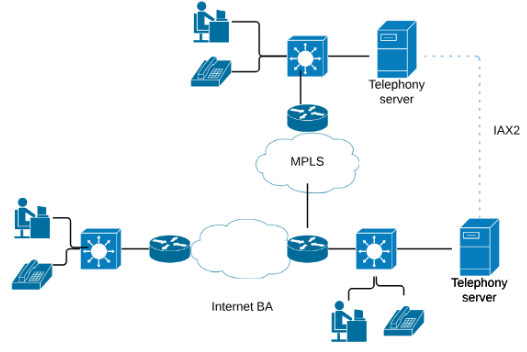
\includegraphics[width=0.9\linewidth]{figure33}}%
%  \subcaptionbox{Another sub-figure\label{fig:rightsubfig}}%
%    {
\includegraphics[width=0.5\linewidth]{knitting-vectorial}}%
  \caption{Telefonía}
  \label{fig:fig2subfig}
\end{figure}

\item[•]\textbf{FTP:}Cada una de las tiendas realiza un proceso de inventariado semanalmente, estos archivos de inventario son subidos a un servidor FTP en la sede nacional de Medellín, por lo tanto el servicio de FTP es considerado como crítico para el negocio.
\item[•]\textbf{Videoconferencia:} el cliente utiliza un servicio de videoconferencia en la nube, más específicamente google Hangouts, que para una calidad óptima de video utiliza 3.2Mbps por videoconferencia, por lo que es una de las aplicaciones que más consumo de ancho de banda genera, es además una de las aplicaciones más críticas para la compañía, ya que es utilizada por los altos directivos.
\item[•]\textbf{CCTV:} el cliente monitorea mediante el enlace de internet de las tiendas, todas la plataforma de CCTV, por lo que se debe garantizar el acceso desde internet a esta aplicación.
\item[•]\textbf{Servicios Web privados:} el cliente cuenta con una Intranet en la que las tiendas y las regionales realizan procesos corporativos vitales para la empresa, de igual forma al hacer parte de un grupo empresarial, consumen en forma de servicios Web aplicaciones en datacenter de otros miembros del grupo empresarial.
\item[•]\textbf{Internet:} desde cada una de las tiendas y las regionales se tiene acceso a internet para navegación, sin embargo este no es un servicio crítico para el cliente.

\item[•]\textbf{Escritorio Remoto:} el grupo de soporte de TI requiere conectividad por escritorio remoto a regionales y tiendas de manera que se pueda realizar un soporte remoto de aplicaciones y equipos de computo.

\item[•]\textbf{Correo:} el cliente cuenta con buzones de correo de google que acceden mediante sus enlaces a internet.
\end{itemize}
Los requerimientos de ancho de banda, jitter y delay así como la criticidad de cada servicio se resumen en la siguiente tabla:

\begin{table}[ht]
	\caption{Amazon EC2 Pricing.}
	\label{tab:hla:results}
\centering
\begin{tabular}{lccccc}
	\toprule
	\multicolumn{1}{c}{\textbf{Proceso}} 	& \textbf{IWAN}	& \textbf{Tiempo}	& \textbf{Solución Actual}
	& \textbf{Tiempo}\\
	\midrule
\cite{Aprovisionamiento tienda nueva} 		& N/A & 2GiB & EBS Only	& \$0.0255 per Hour \\
\cite{a1.large}~2 		& N/A & 4GiB & EBS Only & \$0.051 per Hour	\\
\cite{a1.xlarge}~4		& N/A & 4GiB & EBS Only & \$0.051 per Hour	\\
\cite{a1.2xlarge}~8 	& N/A & 16GiB & EBS Only & \$0.204 per Hour	\\
\cite{a1.4xlarge}~16	& N/A & 32GiB & EBS Only & \$0.408 per Hour	\\
\cite{t3.nano}~2		& N/A & 0.5GiB & EBS Only & \$0.0052 per Hour	\\
\cite{t3.micro}~2   	& N/A & 1GiB & EBS Only & \$0.0104 per Hour	\\
	\midrule
	\textbf{Total}			& \textbf{--}		& \textbf{--}		& \textbf{--} \\
	\bottomrule
\end{tabular}
\end{table}

\section{Requerimientos de Ancho de Banda} % (fold)
\label{sec:Requerimientos de Ancho de Banda}

Con cada una de las aplicaciones descritas se procede a calcular por tanto el ancho de banda requerido en cada una de las sedes, y se genera una estadística del consumo actual en cada una de esas sedes para establecer tanto de manera teórica como práctica el ancho de banda requerido en cada uno de los tipos de sedes remotas y en el centro de datos.
\\
\\
Se realiza un análisis del consumo actual de ancho de banda del cliente utilizando las herramientas de monitoreo disponibles y se obtienen los siguientes datos de consumo para cada una de las 11 sedes regionales y nacionales:
\begin{table}[ht]
	\caption{Amazon EC2 Pricing.}
	\label{tab:hla:results}
\centering
\begin{tabular}{lccccc}
	\toprule
	\multicolumn{1}{c}{\textbf{Proceso}} 	& \textbf{IWAN}	& \textbf{Tiempo}	& \textbf{Solución Actual}
	& \textbf{Tiempo}\\
	\midrule
\cite{Aprovisionamiento tienda nueva} 		& N/A & 2GiB & EBS Only	& \$0.0255 per Hour \\
\cite{a1.large}~2 		& N/A & 4GiB & EBS Only & \$0.051 per Hour	\\
\cite{a1.xlarge}~4		& N/A & 4GiB & EBS Only & \$0.051 per Hour	\\
\cite{a1.2xlarge}~8 	& N/A & 16GiB & EBS Only & \$0.204 per Hour	\\
\cite{a1.4xlarge}~16	& N/A & 32GiB & EBS Only & \$0.408 per Hour	\\
\cite{t3.nano}~2		& N/A & 0.5GiB & EBS Only & \$0.0052 per Hour	\\
\cite{t3.micro}~2   	& N/A & 1GiB & EBS Only & \$0.0104 per Hour	\\
	\midrule
	\textbf{Total}			& \textbf{--}		& \textbf{--}		& \textbf{--} \\
	\bottomrule
\end{tabular}
\end{table}

Con estos datos se puede concluir que ya hay saturación en las sedes, y que por tanto la solución actual está presentando retardos y pérdidas de paquetes en la comunicación.
Se toman muestras de tráfico utilizando el protocolo Netflow con el fin de caracterizar el tráfico de cada una de las aplicaciones obteniendo los siguientes resultados:

\subsection{Sede Nacional Tocancipá:} % (fold)
\label{sec:Sede Nacional Tocancipá:}

\textbf{Ver figura 9.4 Sede Nacional Tocancipá}.
\begin{figure}[htbp]
  \centering
  %\subcaptionbox{\label{fig:leftsubfig}}%
    {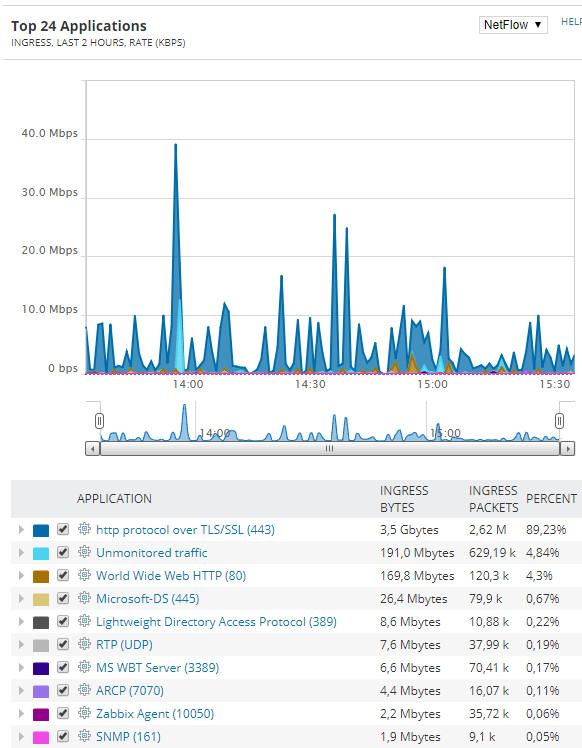
\includegraphics[width=1.0\linewidth]{figure34}}%
%  \subcaptionbox{Another sub-figure\label{fig:rightsubfig}}%
%    {
\includegraphics[width=0.5\linewidth]{knitting-vectorial}}%
  \caption{Sede Nacional Tocancipá}
  \label{fig:fig2subfig}
\end{figure}

\subsection{Sede Nacional Medellín:} % (fold)
\label{sec:Sede Nacional Medellín:}

\textbf{Ver figura 9.5 Sede Nacional Medellín}.
\begin{figure}[htbp]
  \centering
  %\subcaptionbox{\label{fig:leftsubfig}}%
    {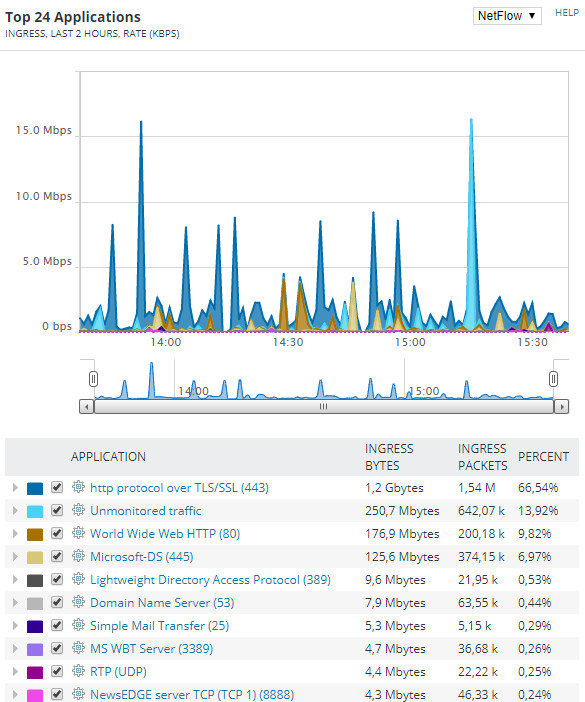
\includegraphics[width=1.0\linewidth]{figure35}}%
%  \subcaptionbox{Another sub-figure\label{fig:rightsubfig}}%
%    {
\includegraphics[width=0.5\linewidth]{knitting-vectorial}}%
  \caption{Sede Nacional Medellín}
  \label{fig:fig2subfig}
\end{figure}

\subsection{Sede Nacional Antioquia Norte:} % (fold)
\label{sec:Sede Nacional Antioquia Norte:}

\textbf{Ver figura 9.6 Sede Nacional Antioquia Norte}.
\begin{figure}[htbp]
  \centering
  %\subcaptionbox{\label{fig:leftsubfig}}%
    {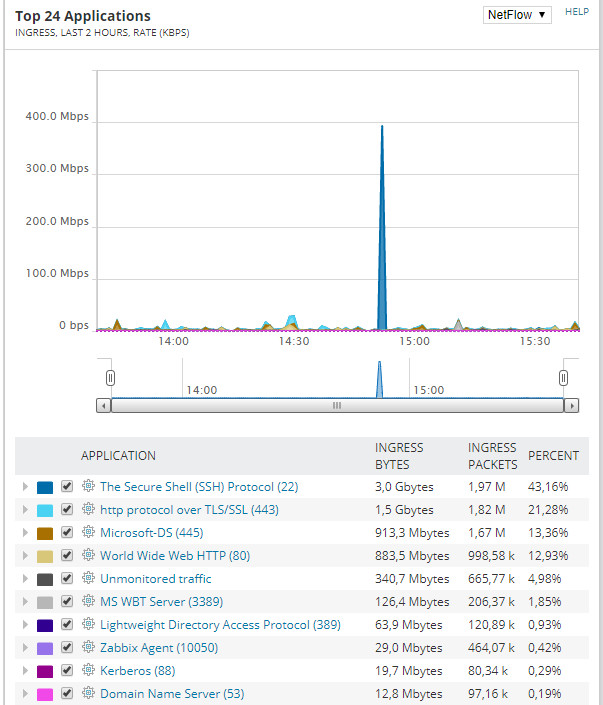
\includegraphics[width=1.0\linewidth]{figure36}}%
%  \subcaptionbox{Another sub-figure\label{fig:rightsubfig}}%
%    {
\includegraphics[width=0.5\linewidth]{knitting-vectorial}}%
  \caption{Sede Nacional Antioquia Norte}
  \label{fig:fig2subfig}
\end{figure}

\subsection{Sede Nacional Antioquia Norte:} % (fold)
\label{sec:Sede Nacional Antioquia Norte:}

\textbf{Ver figura 9.7 Sede Nacional Valle}.
\begin{figure}[htbp]
  \centering
  %\subcaptionbox{\label{fig:leftsubfig}}%
    {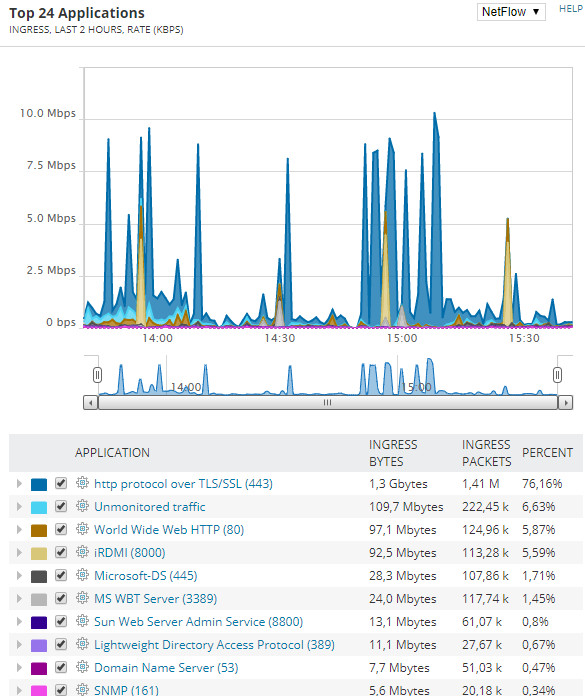
\includegraphics[width=1.0\linewidth]{figure37}}%
%  \subcaptionbox{Another sub-figure\label{fig:rightsubfig}}%
%    {
\includegraphics[width=0.5\linewidth]{knitting-vectorial}}%
  \caption{Sede Nacional Valle}
  \label{fig:fig2subfig}
\end{figure}

De estos resultados se concluye que para todos los casos el Tráfico Web representa la gran mayoría del tráfico que se genera tanto en las regionales como en las sedes nacionales
\\
\\
El tráfico en todos los casos se encuentra al límite de la capacidad, las herramientas de monitoreo no muestran pérdidas de paquetes pero si latencias y jitter que puede afectar la calidad del tráfico de voz y las videoconferencias, adicionalmente en la actualidad no habría posibilidad de crecimiento, teniendo en cuenta el nivel de consumo actual se definen los siguientes anchos de banda para el proyecto:

\begin{table}[ht]
	\caption{Amazon EC2 Pricing.}
	\label{tab:hla:results}
\centering
\begin{tabular}{lccccc}
	\toprule
	\multicolumn{1}{c}{\textbf{Proceso}} 	& \textbf{IWAN}	& \textbf{Tiempo}	& \textbf{Solución Actual}
	& \textbf{Tiempo}\\
	\midrule
\cite{Aprovisionamiento tienda nueva} 		& N/A & 2GiB & EBS Only	& \$0.0255 per Hour \\
\cite{a1.large}~2 		& N/A & 4GiB & EBS Only & \$0.051 per Hour	\\
\cite{a1.xlarge}~4		& N/A & 4GiB & EBS Only & \$0.051 per Hour	\\
\cite{a1.2xlarge}~8 	& N/A & 16GiB & EBS Only & \$0.204 per Hour	\\
\cite{a1.4xlarge}~16	& N/A & 32GiB & EBS Only & \$0.408 per Hour	\\
\cite{t3.nano}~2		& N/A & 0.5GiB & EBS Only & \$0.0052 per Hour	\\
\cite{t3.micro}~2   	& N/A & 1GiB & EBS Only & \$0.0104 per Hour	\\
	\midrule
	\textbf{Total}			& \textbf{--}		& \textbf{--}		& \textbf{--} \\
	\bottomrule
\end{tabular}
\end{table}